\documentclass[12pt,a4paper]{article}
\usepackage{graphicx}
\usepackage{amsmath}
\usepackage{booktabs}
\usepackage{geometry}
\usepackage{hyperref}
\geometry{margin=2.5cm}

\title{PET 212E -- Homework 5\\
\large Core Analysis: Porosity and Permeability Data\\
ITU-PDGM Well-1, Ambient Conditions}
\author{Mert Kaan Akgunlu}
\date{\today}

\begin{document}
\maketitle
\tableofcontents
\newpage

\section{Introduction}
This report presents the core analysis performed on the ITU-PDGM Well-1 dataset for PET 212E Homework 5. The dataset contains petrophysical measurements obtained under ambient conditions and at 800~psi confining pressure, including porosity (both helium and conventional), grain density, air permeability ($K_{air}$), and Klinkenberg-corrected permeability ($K_{\infty}$).

The objectives of this assignment are:
\begin{enumerate}
    \item Plot atmospheric porosity versus grain density and examine the grain density distribution.
    \item Plot 800~psi air permeability versus 800~psi helium porosity on a semi-log scale to observe the permeability--porosity relationship.
    \item Compare 800~psi helium porosity with atmospheric porosity, including a trendline and equality line.
    \item Compare Klinkenberg-corrected permeability ($K_{\infty}$) with air permeability ($K_{air}$) on a log--log scale and quantify the Klinkenberg effect.
\end{enumerate}

\section{Dataset Overview}
The dataset covers 43 core plug samples from a single well. Measurements were taken at ambient conditions (temperature $\approx 25^\circ$C, atmospheric pressure) and under 800~psi confining pressure. Key columns used in this analysis are summarised in Table~\ref{tab:columns}.

\begin{table}[h!]
\centering
\caption{Key petrophysical parameters used in this study.}
\label{tab:columns}
\begin{tabular}{ll}
\toprule
\textbf{Parameter} & \textbf{Description} \\
\midrule
$\phi_{atm}$ & Atmospheric porosity (\%) \\
$\rho_g$     & Grain density (g/cc) \\
$\phi_{He}$  & Helium porosity at 800~psi (\%) \\
$K_{air}$    & Air permeability at 800~psi (mD) \\
$K_{\infty}$ & Klinkenberg-corrected permeability at 800~psi (mD) \\
\bottomrule
\end{tabular}
\end{table}

\section{Results and Discussion}

\subsection{Plot A: Atmospheric Porosity vs.\ Grain Density}
Figure~\ref{fig:plot_a} shows the scatter plot of atmospheric porosity against grain density. A tight cluster around $\rho_g \approx 2.65$~g/cc is consistent with a predominantly quartz-rich (sandstone) lithology. Samples that deviate significantly in grain density may indicate the presence of heavy minerals or authigenic cements.

\begin{figure}[h!]
    \centering
    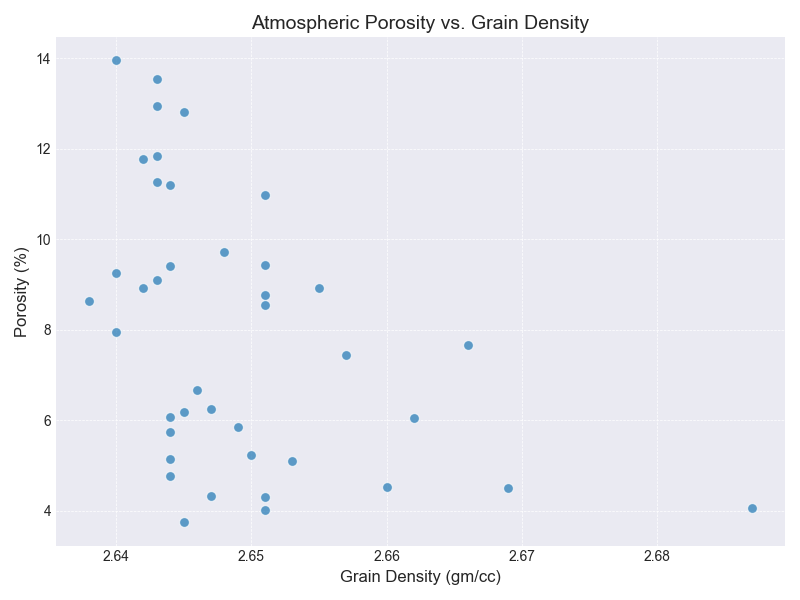
\includegraphics[width=0.8\textwidth]{plot_a.png}
    \caption{Atmospheric porosity vs.\ grain density.}
    \label{fig:plot_a}
\end{figure}

\subsection{Plot B: 800~psi Air Permeability vs.\ 800~psi Helium Porosity (Semi-log)}
Figure~\ref{fig:plot_b} presents the permeability--porosity cross-plot on a semi-logarithmic scale. The positive correlation confirms the expected trend: higher porosity samples generally exhibit higher permeability. The scatter is typical of a heterogeneous reservoir where pore-throat geometry varies independently of total pore volume.

\begin{figure}[h!]
    \centering
    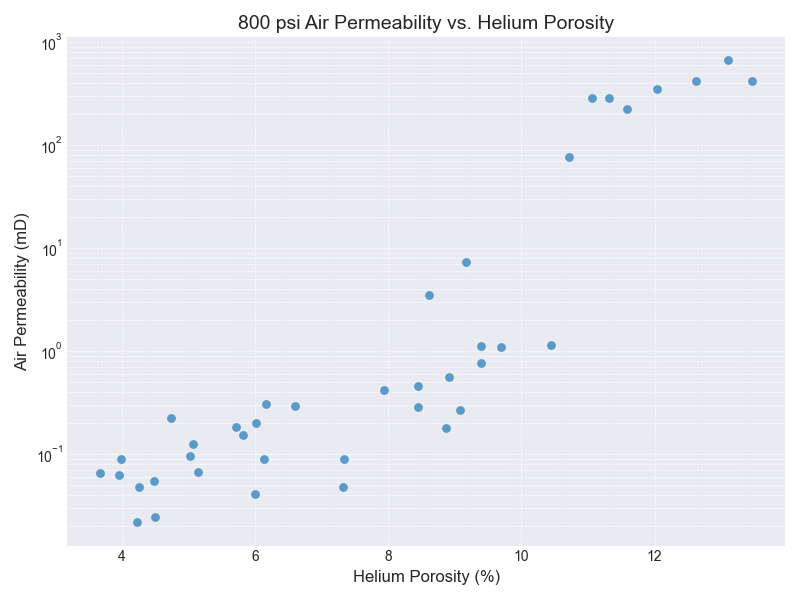
\includegraphics[width=0.8\textwidth]{plot_b.png}
    \caption{800~psi air permeability vs.\ 800~psi helium porosity (semi-log scale).}
    \label{fig:plot_b}
\end{figure}

\subsection{Plot C: 800~psi Helium Porosity vs.\ Atmospheric Porosity}
Figure~\ref{fig:plot_c} compares helium porosity measured at 800~psi confining pressure with atmospheric porosity. The trendline slope is slightly less than 1 (the equality line), indicating that net overburden stress causes measurable pore compaction, reducing effective porosity compared to the unstressed state. The coefficient of determination ($R^2$) quantifies how well 800~psi helium porosity can be predicted from atmospheric measurements.

\begin{figure}[h!]
    \centering
    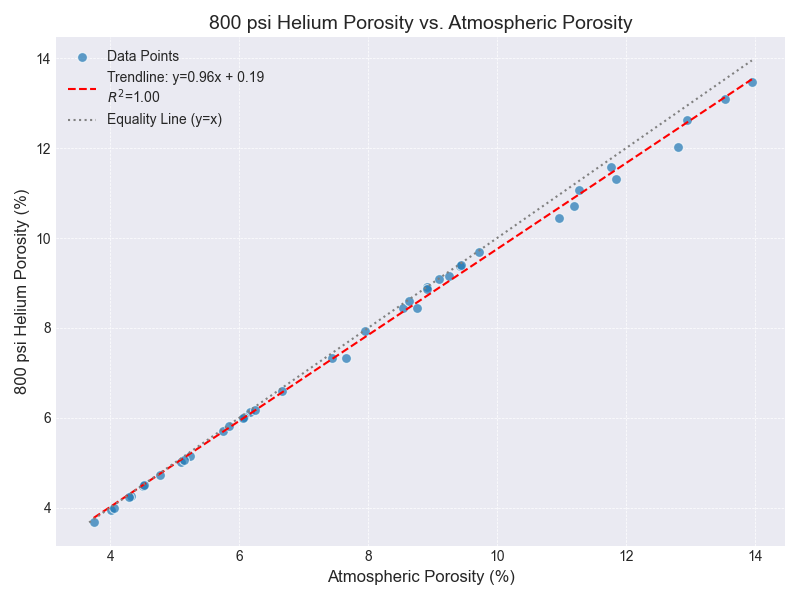
\includegraphics[width=0.8\textwidth]{plot_c.png}
    \caption{800~psi helium porosity vs.\ atmospheric porosity with trendline and equality line.}
    \label{fig:plot_c}
\end{figure}

\subsection{Plot D: $K_{\infty}$ vs.\ $K_{air}$ (Log--Log)}
Figure~\ref{fig:plot_d} compares Klinkenberg-corrected permeability ($K_{\infty}$) with measured air permeability ($K_{air}$) on a log--log scale. Points plotting below the equality line ($K_\infty < K_{air}$) indicate the Klinkenberg effect: gas slippage at low pressure artificially inflates the apparent permeability of tight samples. The power-law trendline quantifies this systematic bias across the permeability range.

\begin{figure}[h!]
    \centering
    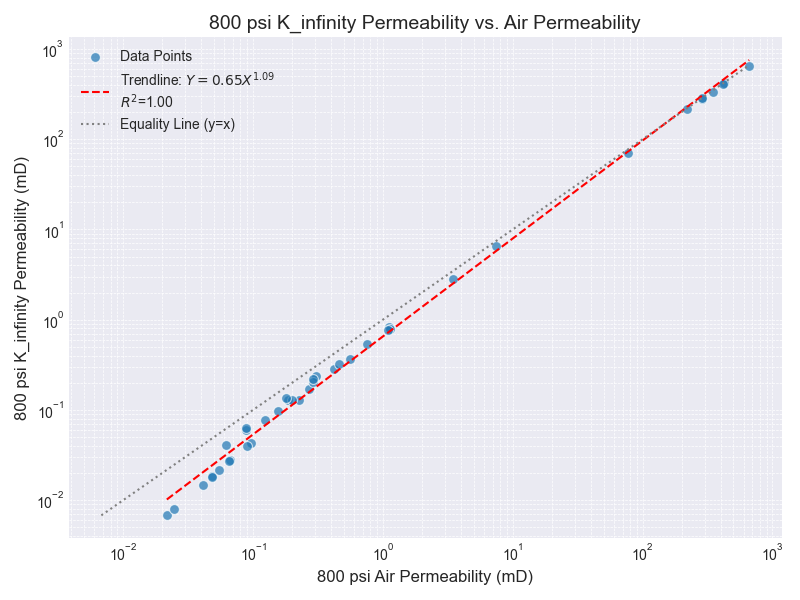
\includegraphics[width=0.8\textwidth]{plot_d.png}
    \caption{Klinkenberg-corrected permeability ($K_{\infty}$) vs.\ air permeability ($K_{air}$) on a log--log scale.}
    \label{fig:plot_d}
\end{figure}

\section{Conclusion}
The core analysis of ITU-PDGM Well-1 data confirms:
\begin{itemize}
    \item The formation is dominated by quartz-rich mineralogy ($\rho_g \approx 2.65$~g/cc).
    \item A positive permeability--porosity correlation exists, though pore-geometry heterogeneity introduces scatter.
    \item Confining stress (800~psi) reduces porosity compared to atmospheric measurements, as expected from pore compaction.
    \item The Klinkenberg effect is significant in low-permeability samples, where $K_{air}$ overestimates $K_{\infty}$ by a measurable margin.
\end{itemize}

\end{document}
